% lint-skip: 未完成ステータス（figure/table caption 未対応，人手チェック時に解消予定）
\documentclass[../../main.tex]{subfiles}
\begin{document}

\begin{flushright}
  \footnotesize\textit{【自動文字起こし・要確認】}
\end{flushright}

[解] $P$は$
\begin{pmatrix} 2 \\ 2t
\end{pmatrix}, Q
\begin{pmatrix} 1 \\ t
\end{pmatrix}$から,
$PQ : \dfrac{1}{2}x - (t+1)\cdot\dfrac{1}{2}t - (y-t) = 0$
とおける. セイリして
$$ t^2 - xt + y = 0 \quad \cdots \text{\textcircled{1}} $$
をみたす$t \in \mathbb{R}$が存在するので, 判別式$D$として$D \ge 0$.
$$ x^2 - 4y \ge 0 $$
これを図示して, 右図斜線部.
\begin{figure}[htbp]
  \centering
  \begin{tikzpicture}[x=1.15cm,y=1.15cm,>=stealth]
    \fill[blue!9] (-2.2,-1.1) rectangle (2.2,1.21);
    \fill[white] (-2.2,1.21)--(-2.2,1.21)
    plot[domain=-2.2:2.2,samples=80] (\x,{0.25*\x*\x})--(2.2,1.21)--cycle;
    \draw[->,gray!75] (-2.4,0)--(2.5,0) node[right] {$x$};
    \draw[->,gray!75] (0,-1.2)--(0,1.65) node[above] {$y$};
    \draw[blue!75!black,very thick,domain=-2.2:2.2,samples=80]
    plot (\x,{0.25*\x*\x});
    \node[above right,blue!75!black] at (1.35,0.7) {$y=\dfrac{x^2}{4}$};
    \node[below right] at (0,0) {$O$};
    \node[blue!75!black] at (-1.35,-0.55) {$D\geq 0$};
  \end{tikzpicture}
  \caption{判別式 $D=x^2-4y\geq0$ を満たす領域}
\end{figure}

\paragraph{(2)}

\textcircled{1}から
$y = f(t) = -t^2 + xt \quad (0 \le t \le 1, \ t-1 \le x \le t+1)$
をみたす$(x,y)$をもとめる. $x=X$と固定し, 右辺$g(t)$の値域をもとめる. $(X-1 \le t \le X+1)$ 右図から
\begin{figure}[htbp]
  \centering
  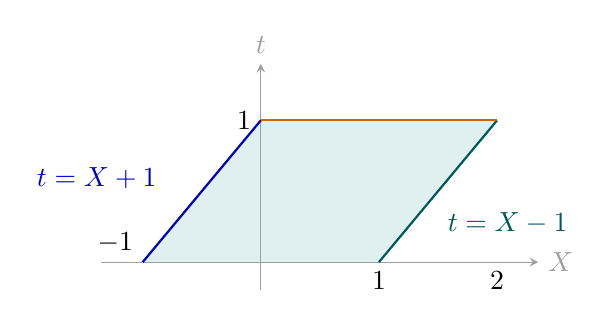
\begin{tikzpicture}[x=1.5cm,y=1.8cm,>=stealth]
    \fill[teal!12] (-1,0)--(0,1)--(2,1)--(1,0)--cycle;
    \draw[->,gray!75] (-1.35,0)--(2.35,0) node[right] {$X$};
    \draw[->,gray!75] (0,-0.2)--(0,1.4) node[above] {$t$};
    \draw[blue!75!black,thick] (-1,0)--(0,1);
    \draw[teal!70!black,thick] (1,0)--(2,1);
    \draw[orange!80!black,thick] (0,1)--(2,1);
    \node[above left] at (-1,0) {$-1$};
    \node[below] at (1,0) {$1$};
    \node[below] at (2,0) {$2$};
    \node[left] at (0,1) {$1$};
    \node[above left,blue!75!black] at (-0.8,0.45) {$t=X+1$};
    \node[below right,teal!70!black] at (1.5,0.42) {$t=X-1$};
  \end{tikzpicture}
  \caption{$0\leq t\leq1$ と $t-1\leq X\leq t+1$ の範囲}
\end{figure}
$$
\begin{cases}
  g\left(\dfrac{X}{2}\right) \ge y \ge g(1) & (0 \le X \le 2) \\
  g(0) \ge y \ge g(X+1) & (-1 \le X \le 0)
\end{cases}
$$
だから$X$をうごかして
$$
\begin{cases}
  -x-1 \le y \le 0 & (-1 \le x \le 0) \\
  x-1 \le y \le \dfrac{1}{4}x^2 & (0 \le x \le 2)
\end{cases}
$$
より, この領域は右図斜線部 (境界含む) で, もとめる面積は
\begin{align}
  S &= \dfrac{1}{2} \cdot 1 \cdot 1 + \int_0^2 \left(\dfrac{1}{4}x^2 - x + 1\right) dx \\
  &= \dfrac{1}{2} + \dfrac{1}{3} \cdot \dfrac{1}{4} \cdot 2^3 \\
  &= \dfrac{7}{6} \quad \text{\#}
\end{align}

\begin{figure}[htbp]
  \centering
  \begin{tikzpicture}[x=1.45cm,y=1.45cm,>=stealth]
    \fill[teal!16] (-1,0)--(0,0)--plot[domain=0:2,samples=60]
    (\x,{0.25*\x*\x})--(0,-1)--cycle;
    \draw[->,gray!75] (-1.35,0)--(2.5,0) node[right] {$x$};
    \draw[->,gray!75] (0,-1.3)--(0,1.45) node[above] {$y$};
    \draw[blue!75!black,very thick,domain=0:2,samples=60]
    plot (\x,{0.25*\x*\x});
    \draw[orange!85!black,thick] (-1,0)--(0,-1)--(2,1);
    \draw[blue!75!black,thick] (-1,0)--(0,0);
    \node[above left] at (-1,0) {$-1$};
    \node[below] at (2,0) {$2$};
    \node[below left] at (0,-1) {$-1$};
    \node[above left,blue!75!black] at (1.55,0.62) {$y=\dfrac{x^2}{4}$};
    \node[below right,orange!85!black] at (0.95,-0.6) {$y=x-1$};
  \end{tikzpicture}
  \caption{面積 $S$ を求める領域（境界を含む）}
\end{figure}

\end{document}
